\documentclass[../main.tex]{subfiles}
\begin{document}
    
    \begin{frame}
        \frametitle{2: Marker detection (wall scene)}
        \begin{figure}[!htb]
            \centering
            \subfloat[\small{ps3-2-a-1}]{\frame{
\includegraphics[keepaspectratio,height=0.65\textheight,width=0.45\textwidth]{ps3-2-a-1}} } \hspace{3em}
            \subfloat[\small{ps3-2-a-2}]{\frame{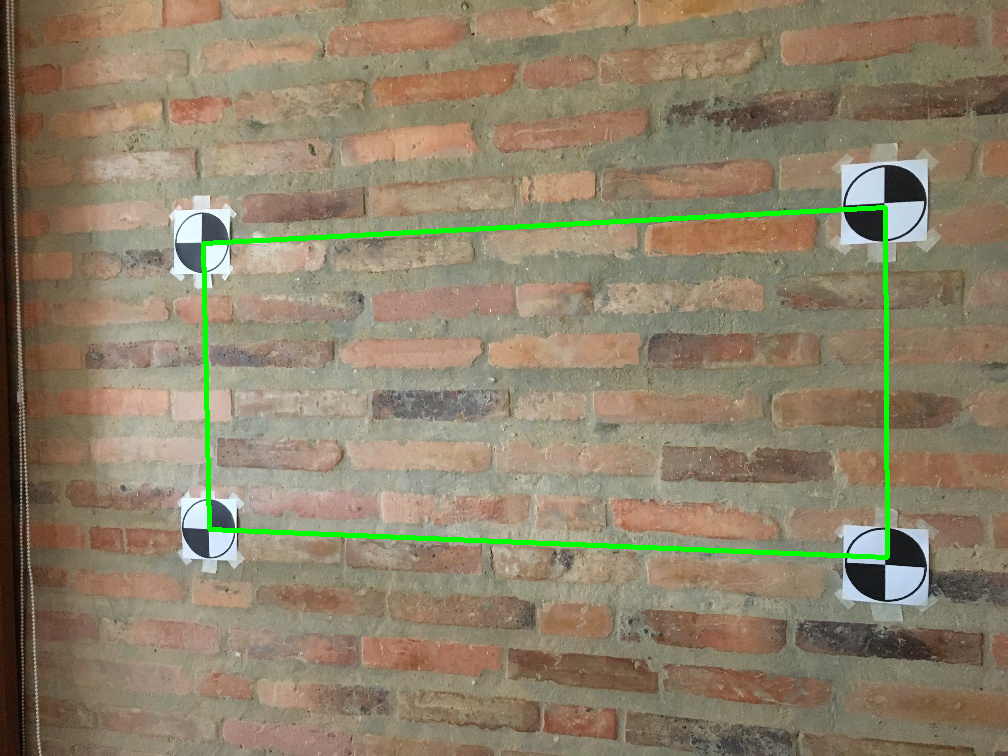
\includegraphics[keepaspectratio,height=0.65\textheight,width=0.45\textwidth]{ps3-2-a-2}}}
        \end{figure}
    \end{frame}

    \begin{frame}
        \frametitle{2: Marker detection (wall scene)}
        \begin{figure}[!htb]
            \centering
            \subfloat[\small{ps3-2-a-3}]{\frame{
\includegraphics[keepaspectratio,height=0.65\textheight,width=0.45\textwidth]{ps3-2-a-3}} } \hspace{3em}
            \subfloat[\small{ps3-2-a-4}]{\frame{
\includegraphics[keepaspectratio,height=0.65\textheight,width=0.45\textwidth]{ps3-2-a-4}}}
        \end{figure}
    \end{frame}

    \begin{frame}
        \frametitle{2: Marker detection (wall scene)}
        \begin{figure}[!htb]
            \centering
            \frame{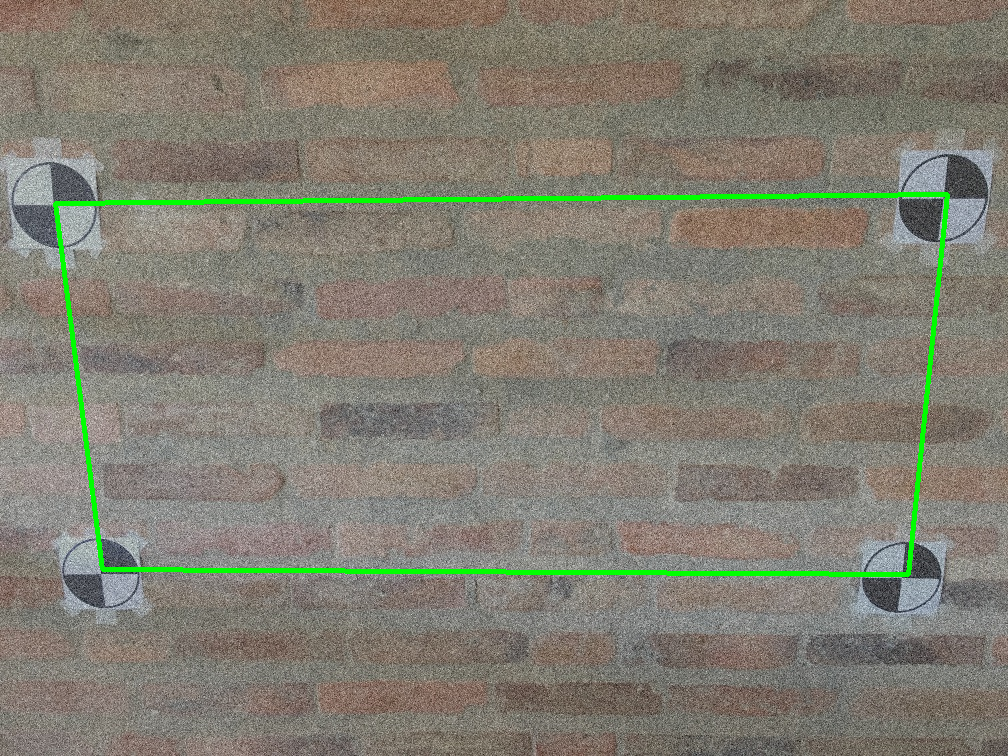
\includegraphics[keepaspectratio,height=0.65\textheight,width=0.45\textwidth]{ps3-2-a-5}}
            \caption{ps3-2-a-5} 
        \end{figure}    
    \end{frame}
    
\end{document}